\chapter{Fundamentação}
Construir uma aplicação que reaja de forma apropriada a sentenças de uma dada linguagem é necessário um reconhecedor que identifique uma gramática que é um conjunto de regras as quais sentenças desta linguagem são submetidas. Analogamente pode-se comparar sentenças de um linguagem de programação com sentenças de algum idioma como português onde faz-se necessário identificar classes como sujeito, predicado e objeto para entender e agir de maneira adequada. Desta forma quando uma sentença como \texttt{public int x = 10;} é inserida em algum reconhecedor este deve se dotado de algum mecanismo que possibilite identificar as subpartes da sentença para que a aplicação reaja de acordo com as regras gramaticais da linguagem. Como exemplo de reconhecedor tem-se a calculadora que reage de forma adequada as sentença válida na entrada.

Para atingir o objetivo do trabalho de conclusão de curso também foi necessário compreender temas relacionados à evolução da linguagem Java, engenharia de linguagens de software (ou do Inglês \emph{Software Language Engineering}). Para fornecer uma introdução ao leitor, este capítulo apresenta uma visão geral sobre esses temas. Note que não foi objetivo deste trabalho implementar um mecanismo de transformação de código, mas sim construir um suporte ferramental efetivo para compreender como os desenvolvedores usam as construções existentes na linguagem Java e \emph{identificar oportunidades de melhoria de código}, algo essencial para permitir a atualização de um código existente que utilize construções ultrapassadas de uma linguagem de programação.

Devido a necessidade do \NOMESOFTWARE possuir um reconhecedor para linguagem Java, a contextualização do leitor é necessária tendo em vista a complexidade inerente da construção de uma aplicação que reconheça e manipule linguagens de programação. Caso o leitor tenha pleno conhecimento dos passos necessários para a manipulação de linguagem de programação pode ir diretamente para o próximo capítulo \ref{cap:arquiteruta} que é a explicação detalhada da arquitetura deste trabalho. 

Somente com exceção da Seção \ref{sec:evolucaoJava} as demais seções deste capítulo seguem a mesma ordem que o \NOMESOFTWARE  utiliza para pesquisar características na linguagem Java. A Seção \ref{sec:evolucaoJava} trata do histórico evolutivo de características da linguagem Java pertinente a este trabalho. Nas Seções \ref{sec:parser} e \ref{sec:rec} serão evidenciadas características para realizar a representação intermediária de uma linguagem de programação, a Seção \ref{sec:softEng} evidenciará conceitos relativos a engenharia de linguagens de programação,  a Seção \ref{sec:visitor} explicará características necessárias para pesquisar estruturas na representação intermediária e a Seção \ref{sec:as} abordará o conceito de análise estática.

\section{Evolução da Linguagem Java}\label{sec:evolucaoJava}
No início dos anos noventa, um grupo de engenheiros da Sun Microsystems, chamados de \textit{Green Team}, acreditava que a próxima grande área da computação seria a união de equipamentos eletroeletrônicos com os 
computadores. O \textit{Green Team}, liderado por James Gosling, especificou a linguagem de programação Java, 
inicialmente proposta para dispositivos de entretenimento como aparelhos de TV a cabo. Por outro lado, apenas em \num{1995}, com a massificação da Internet, a linguagem Java teve sua primeira grande aplicação: a construção de componentes de software para o navegador \textit{Netscape}.

Java é uma linguagem de programação de propósito geral, orientada a objetos e concebida para ser independente de plataforma, por fazer uso de uma máquina virtual: a \emph{Java Virtual Machine} (JVM). Isso permite que uma aplicação Java possa ser executada em qualquer ambiente computacional que possui uma JVM aderente à especificação da linguagem.

Na sua primeira versão publicamente disponível (\acs{JDK} 1.0.2), existiam apenas oito bibliotecas presentes na especificaçã Java, tais como \texttt{java.lang}, \texttt{java.io}, \texttt{java.util},  
\texttt{java.net}, \texttt{java.awt} e \texttt{java.applet}; onde as três últimas favoreciam a construção de soluções envolvendo mobilidade de código: um componente (um \textit{applet} Java) poderia ser transferido de um servidor para um cliente e, dessa forma, ser executado em um navegador Web compatível. As características de independência de plataforma e a aproximação com a Web fez com que a linguagem Java se tornasse bastante popular, passando a ser usada em outros domínios (como o desenvolvimento de software 
para cartões inteligentes, para jogos eletrônicos e para ambientes corporativos) e a ter uma evolução natural com a melhoria de desempenho da JVM e a incorporação de um conjunto significativo de  bibliotecas. 


Apesar de toda essa evolução, que trouxe uma rápida aceitação da linguagem, mudanças significativas na especificação da semântica da linguagem só se tornaram publicamente disponíveis em 2004, com o lançamento da versão intitulada Java 5.0 (\emph{Java Language Specification 1.5}). As principais contribuições para a semântica da linguagem afetavam diretamente a produtividade dos desenvolvedores e incluíam implementações mais eficientes de bibliotecas existentes (como as bibliotecas de IO e as bibliotecas para programação concorrente). Relacionadas à perspectiva semântica, as principais contribuições da especificação Java 5.0 introduziram o suporte a polimorfismo parametrizado (Java Generics) e enumerações; o uso de construções \texttt{foreach} para iterar sobre coleções; a possibilidade de definição de múltiplos argumentos com a construção \texttt{varargs} (suportados em linguagens como C); e o uso do mecanismo intitulado \emph{autoboxing} para converter tipos primitivos nas classes Java correspondentes. 

As versões da linguagem Java 7 e Java 8 também trouxeram, 
em maior ou menor grau de significância, extensões sintáticas 
e semânticas bastante aguardadas pela comunidade de 
desenvolvedores, tais como:

\begin{description}
\item[Java 5] ....

\item[Java 7] introduziu em 2011 facilidades como (a) suporte ao tipo \texttt{String} 
em sentenças condicionais \texttt{switch}, (b) inferência de tipos 
na instanciação de classes genéricas e (c) captura de 
múltiplos tipos de exceção. 

\item[Java 8] introduziu em 2014 o suporte a expressões lambda e a implementação de 
métodos \emph{default} em interfaces Java. O suporte a expressões lambda pode 
ser compreendido como uma evolução da linguagem tão significativo 
quanto a introdução de Java Generics, na versão Java 5. Isso porque 
uma série de novos idiomas (baseadas em \emph{streaming} para programação 
concorrente) estão sendo propostos para a linguagem com base em tal construção.   
\end{description} 


\section{Sentenças de uma linguagem}
Toda linguagem de programação é composta por sentenças válidas que respeitam uma regra bem definida onde esta regra é semelhante a gramática presente em qualquer idioma.  Esta sentenças são compostas por frases onde cada frase pode é definida por uma conjunto de sub-frases e símbolos que compõem o vocabulário desta linguagem. 
%Como analogia tem-se a língua falada... No computador não é diferente este somente executa sentenças que podem ser interpretadas corretamente

Quando símbolos são agrupados corretamente tem-se as frases da linguagem que serão convertida em instruções de máquina. Similar a uma idioma como inglês ou português onde o vocabulário é composto por verbos, nomes e outras classes, a linguagem de programação não é diferente, o vocabulário possui símbolos com diferentes regras para poder efetuar a comunicação com o computador e estas podem ser variáveis, operadores outros. Pode-se identificar uma sequência como a seguinte expressão \textit{if x<0 then x = 0;} e a Figura~\ref{fig:rep_intermediaria} exemplifica a representação intermediária de uma linguagem segundo explica Terrance Parr~\cite{Parr:2009:LIP:1823613}.


\begin{figure}[ht]
\centering
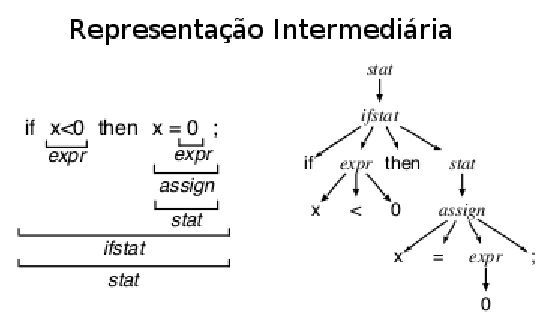
\includegraphics[scale=1]{Imagens/rep_intermediaria}
\label{fig:rep_intermediaria}
\caption{Reconhecimento de sentenças de uma linguagem.}
\end{figure}

A Figura \ref{fig:rep_intermediaria} exibe um primeiro estágio onde é realizada uma agrupamento de classes que compõem a sentença e um segundo estágio que é a elaboração da representação intermediária preservando a hierarquia das classes e símbolos que foram definidos na gramática da linguagem.


\section{Reconhecedores}\label{sec:rec}
Reconhecedores são dispositivos formais com especificações finitas que permitem verificar se uma dada sentença é válida ou não. Vale ressaltar que os símbolos isolados são considerados unidades atômicas. A linguagem Java proporciona uma flexibilidade para estes mecanismos pois é possível reconhecer seus símbolos por ter como entrada o código fonte Java ou \textit{bytecode} gerado após a transformação do código fonte.

Os reconhecedores de gramática são denominados \textit{parsers} ou analisadores sintáticos pois reagem de forma adequada a um idioma específico. Devido a complexidade de implementar uma ferramenta desta natureza é necessário dividir a tarefa tomando por base a leitura de uma pessoa que ao ler uma sentença não ler caractere por caractere mas sim um fluxo de palavras. Desta forma a tarefa de leitura é dividida em duas partes a primeira agrupa palavras de acordo com a classe que ela representa e a segunda por reconhecer o sentido que a palavra possui. 

Quando um reconhecedor tem a entrada válida inicia-se o primeiro estágio que é agrupar os símbolos ou palavras da linguagem, este processo de agrupar é denominado análise léxica ou apenas \textit{tokenizing}. Este agrupamento léxico pode ser realizado por classes de \textit{tokens} ou por tipos, \texttt{INT, FLOAT} ou outros. O segundo estágio é gerar uma representação para os grupos reconhecidos. Neste trabalho a representação é realizada através de uma árvore de sintaxe abstrata que será detalha da próxima Seção \ref{sec:parser}. A Figura \ref{fig:rep_intermediaria} exemplifica a separação dos tipos gramaticais e a representação intermediária.


%Para implementar ou identificar qualquer sentença é necessário a contrução de um programa capaz aceitar tais sentenças como entrada e reagir de forma apropriada. Tendo em vista que uma linguagem é um conjunto de sentaças válidas

%As aplicações pesquisam ou manipulam estruturas de uma linguagem tem a necessidade de  reconhecer entradas que é a sintaxe da linguagem para prover uma saída desejada, tais aplicações são denominadas aplicações de sintaxe direta pois geram uma saída dado o reconhecimento de uma entrada válida. Um simples exemplo é a necessidade de traduzir um formato específico de linguagem de marcação para HTML, é necessário de alguma forma reconhecer entradas e traduzi-las para a saída desejada, neste exemplo páginas HTML.

\section{Representação Intermediária}\label{sec:parser}
Após todo reconhecimento das sentenças pertencentes a linguagem é necessário criar um mecanismo que terne automático a elaboração da representação intermediária de cada arquivo fonte. Esta representação deve possuir duas características importantes. A primeira é ser de fácil construção para representar as sequências de entrada e a segunda é possibilitar de forma fácil a navegação nesta estrutura para identificar as mais diversas construções que uma linguagem pode conter. Vale ainda ressaltar que representação da linguagem Java gerada neste trabalho possui a mesma equivalência do código fonte o que permite a pesquisa de construções específicas. 

Para a criação desta representação foi utilizada a biblioteca Eclipse-JDT a qual facilita a criação desta representação por possuir um vasto conjunto de classes que facilitam a criação e pesquisa na árvore sintática gerada nas mais diversas versões existente da linguagem, cabe ainda destacar que a biblioteca Eclipse-JDT possui representação para outras linguagens além de Java o que acarreta em poder utilizar outra linguagem como objeto de pesquisa além de Java.
 
Para que realização da transformação de linguagem ocorra neste nível é necessário um mecanismo que crie uma representação intermediária da linguagem e para que isto faz-se necessário que exista um reconhecedor onde este é responsável por identificar as frases que compõem os códigos fontes. Vale ressaltar que as frases são as sentenças declaradas nos arquivos fontes.

A concepção de uma representação ocorra é necessário que aconteça algumas etapas básicas antes da representação ser realizada e estas etapas são a correta identificação da linguagem a ser manipulada através de um reconhecedor que identificam as frases que compõem a linguagem. Essas frases são todas as sentenças declaradas nos arquivos fontes.


\section{Navegação na Representação Intermediária}\label{sec:visitor}
Conforme mencionado no capítulo de introdução, o principal objetivo deste trabalho de conclusão de curso é identificar oportunidades de evolução de código  em projetos que utilizam recursos anteriores aos disponíveis nas versões 7 e 8 da linguagem Java, algo necessário para o contexto de reestruturação de código que visa adequar um código existente a construções mais atuais. Importante destacar que as versões da linguagem Java mencionadas anteriormente introduziram novos recursos, tais como: \texttt{multi-catch}, \texttt{try-with-resource}, \texttt{switch-string} e \texttt{lambda expressions}.
% e que esse tipo de evolução constitui uma nova perspectiva de refatorar, que é caracterizado por uma transformação de código que preserva comportamento e que passa a usar  novas construções da linguagem de programação \cite{Overbey:2009}).

Para concretizar o objetivo deste trabalho foi necessário utilizar um algoritmo que realize uma operação de visitar os elementos da árvore de sintaxe abstrata que é a representação intermediária explicada na seção anterior \ref{sec:parser}. Para tal tarefa foi adotado o padrão de projeto \textit{Visitor} elaborado por Gamma et. al.\cite{Gamma:1995} devido a característica de permitir que seja criada uma nova operação sem que seja necessário modificar a classe dos elementos as quais são operados. Devido a tal característica torna-se razoavelmente fácil navegar entre os nós da árvore sintática e pesquisar por construções dado a classe gramatical desejada. Destaca-se ainda que a biblioteca Eclipse-JDT utilizada para gerar a representação intermediária também prove inúmeros \textit{Visitors} para pesquisar as mais diversas características.


%Para atingir o objetivo do trabalho de conclusão de curso, foi necessário compreender temas relacionados à evolução da linguagem Java, engenharia de linguagens de software (ou no Inglês \emph{Software Language Engineering}) e refatoramento de código (\emph{code refactoring}). Para fornecer uma introdução ao leitor, este capítulo apresenta uma visão geral sobre esses temas. Note que não foi objetivo deste trabalho implementar um mecanismo de transformação de código, mas sim construir um suporte ferramental efetivo para compreender como os desenvolvedores usam as construções existentes na linguagem Java e \emph{identificar oportunidades de melhoria de código}, algo essencial para permitir a atualização de um código existente que usa construções ultrapassadas de uma linguagem de programação.


\section{Engenharia de Linguagens de Software}\label{sec:softEng}


%\begin{flushright}
%\emph{
%\ldots ou engenharia de software para linguagens de programação 
%(no Inglês, Software Language Engineering).}
%\end{flushright}

A manipulação de artefatos escritos em 
uma linguagem de programação (ou em linguagens de software) 
é uma tarefa desafiadora, mas que permite o desenvolvimento 
de software aplicável a diferentes cenários, como, por exemplo, 
manipular arquivos \texttt{XML}, transformar 
informações e scripts presentes 
em bancos de dados legados, efetuar a tradução de programas 
escritos em uma versão desatualizada de uma linguagem. 

Por envolver diferentes estágios, o desenho desse tipo de solução requer, geralmente, 
um estilo arquitetural baseado em um \emph{pipeline},  onde cada estágio necessário à  
 manipulação de uma linguagem é implementado como um componente de software. Quando combinados, 
tais componentes constituem uma solução que realiza o processamento 
de uma ou mais linguagens. A Figura~\ref{fig:stagesLanguageApp} exibe uma organização 
típica de componentes para o processamento de artefatos escritos em uma linguagem de 
programação, onde a cada estágio do \emph{pipeline}, um componente 
utiliza os resultados do estágio anterior para gerar uma saída para o componente 
que realiza o processamento no estágio posterior.  

\begin{figure}[h]
  \center
  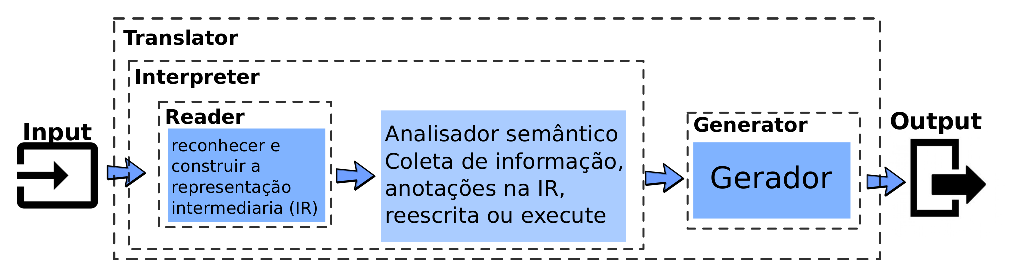
\includegraphics[scale=0.9]{Imagens/stagesLanguageApp}
  \label{fig:stagesLanguageApp}
  \caption{Fases de aplicações com linguagens.}
\end{figure}

Existe uma forte relação entre a engenharia de linguagens de programação e a construção típica de um software, onde as aplicações deste domínio compreendem \texttt{reconhecedores, interpretadores, tradutores e geradores}~\cite{Parr:2009:LIP:1823613}. 

\begin{description}

\item[Reconhecedor] é uma construção capaz de receber uma estrutura de dado como um input ou um fluxo de inputs. O fluxo de input pode geralmente é texto puro mas pode ser utilizado dado binário. Como exemplo de aplicação tem-se ferramentas analisadoras de referências cruzadas, e ferramentas para carregar classes.

\item[Interpretador] Um interpretador, lê uma entrada, decodifica e executa as instruções, interpretadores variam de simples calculadoras até a implementação de linguagens de programação como Java, Python e PHP.

\item[Tradutor]A partir um input de texto ou binário é emitido uma saída para uma linguagem que pode ser a mesma ou não. É a combinação do \textit{reader} e \textit{generator}. Como exemplo tem-se tradutores de linguagens extintas para linguagens atuais, \texttt{refactorers},  gerador de logs e macro pre-processadores.
	
\item[Gerador] Percorre uma estrutura de dado e emite uma saída. Como exemplo tem-se ferramentas de mapeamento de objetos relacionais em banco de dados, serializador de objetos, gerador de código fonte e geradores de página web.

\end{description}


Além dessas aplicações típicas, ferramentas para a identificação estática de \emph{bugs}, por exemplo, também são comumente implementadas usando uma organização como a representada na Figura~\ref{fig:stagesLanguageApp}. A ferramenta \textit{FindBugs}~\cite{FindBugs} serve como um exemplo de solução para identificação  de possíveis erros em programas escritos na linguagem Java, a partir do \emph{bytecode} resultante do processo de compilação. Note na Figura~\ref{fig:findBugs} a semelhança arquitetural com as abordagens típicas para o processamento de artefatos de linguagens de programação. 

\begin{figure}[h]
	\center
	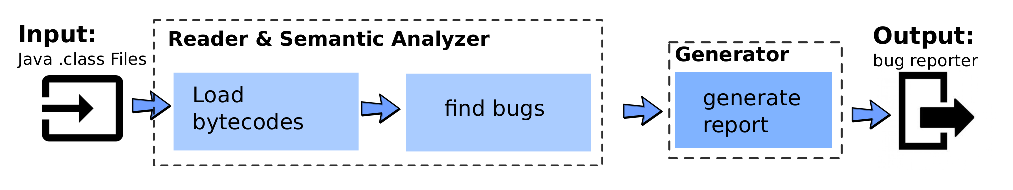
\includegraphics[scale=0.9]{Imagens/pipelineFindbugs}
	\label{fig:findBugs}
	\caption{Fases do pipiline do FindBugs.}
\end{figure}


Especificamente no caso deste trabalho, percebeu-se a necessidade de construção de um software que 
realiza a análise estática de código para identificar tanto o uso quanto as oportunidades do uso de construções 
sintáticas / semânticas da linguagem Java. Em termos arquiteturais, a Figura~\ref{fig:stagesAnalyzer} ilustra, 
em um alto nível de abstração, os principais componentes que formam o \emph{pipeline} do analisador estático 
implementado nesse trabalho e cujos detalhes de implementação são apresentados no próximo capítulo.

\begin{figure}[h]
	\center
	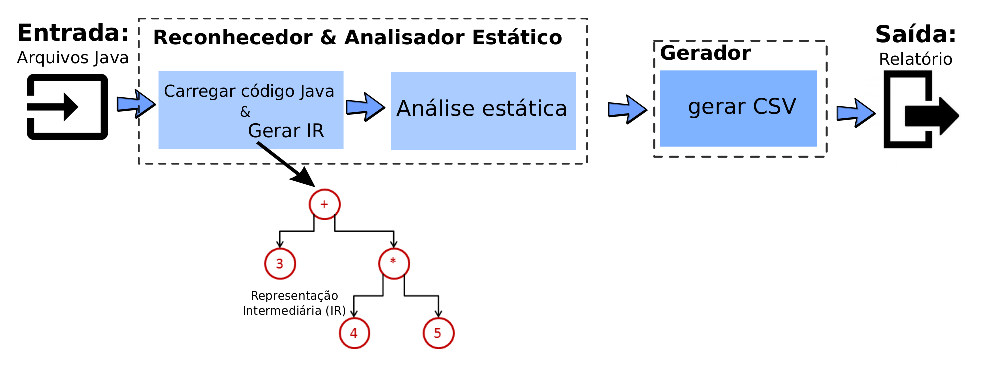
\includegraphics[scale=0.9]{Imagens/stagesAnalizer}
	\label{fig:stagesAnalyzer}
	\caption{Ferramentas necessárias para construção do analisador estático.}
\end{figure}


Pode-se compreender este analisador como um \emph{grammarware}, pois é um software 
que depende fortemente de uma gramática para seu funcionamento; neste caso a gramática da linguagem Java. 
%\emph{Grammawares} demandam um conhecimento essencial das  gramáticas que manipulam. 
%Como exemplos de arquiteturas que possuem tal conhecimento tem-se os programas de conversão de dados, processadores de \texttt{XML} e os que efetuam \textit{parses}.
De acordo com Paul Klint et al.~\cite{klint2005toward}, alguns cenários favorecem o desenvolvimento de softwares alinhados com a abordagem 
\emph{grammarware}, com destaque às aplicações que necessitam importar perfis de usuários para promover a transição da versão 
antiga para uma versão nova. 
Esta transição deve ser robusta e provavelmente necessitará de adptação deverá passar 
por um parser para que as partes que necessitem de adaptação possam ser identificadas.

Um outro cenário real é o desenvolvimento de aplicações de banco de dados onde se faz necessário adotar 
uma nova linguagem de definição para um ambiente específico. De forma que automatizar esta solução requer o uso de um 
parser que será responsável por reconhecer as entradas necessárias para efetuar o mapeamento 
para a \emph{linguagem} destino.


%% Um \textit{software} que efeta manipulação da gramática de uma linguagem, como no caso deste trabalho de conclusão fica evidente o aparecimento da questão sobre \textit{refactoring} e dentre diversas caracterísitas explicadas por Martin Fowler~\cite{martinFowlerRafactoring}, fica claro que este trabalho contribui com o intu\'{\i}to de identificar construções obsoletas não efetuando \textit{refactoring} automático mas fazendo  com que o desenvolvedor opte pela evolução ou não. Pois a evolução do código por um mais atual é uma das oportunidades de melhorar o desgin do \textit{software} conforme aborda por Martin Fowler~\cite{martinFowlerRafactoring} em seu livro.

%% Mesmo sem a implementação de \textit{refactoring} uma contribuição que este trabalho faz é a identifição a capacidade de encontrar código duplicado como por exemplo ao identificar \texttt{catch} repetidos, ou até mesmo melhorar o desempenho com no caso da da utilização do \texttt{switch-string} ao invés do \texttt{if-string} pois oracle afirma que o desempenho é melhor de a implementação otimizada do \texttt{switch-string} na documentação~\cite{docSwitch}.




%Atualmente a evolução de uma linguagem de programação ocorre predominantemente de forma {\it ad-hoc} e em muitos casos manualmente, para a tradução de aplicativos legados, conforme a demanda. A ferramentas de análise para gerar a evolução necessária, {\it grammarware}, tende a condizir este processo abordando a classe gramatical que deve ser evoluída. Neste caso analisador que muitas vezes realizaria o trabalho por tentativa e erro, tem como base a gramática do código a ser analisado. Especificações do analisador são derivados automaticamente da semi gramática. Diferentes tecnologias de análise que podem ser orientadas em oposição a uma tecnologia específica. Assim o processo de personalização/evolução é susceptível de exigir a entrada de um engenheiro de {\it grammarware} o qual tem conhecimento prévio da gramática a ser analisada.

%Um ponto crítico quanto a análise de código fonte é o \textit{parser} da linguagem, onde é necessário reconhecer uma frase para efetuar a interpretação ou fazer a tradução para que a criação da representação intermediária aconteça. Inicialmente é necessário identificar se a frase que será tratada é um \textit{assignment} ou uma chamada de função.
 
%Reconhecer uma frase acarreta em duas coisas, distingui-la de outras construções e identificar os elementos e as subestruturas que compõem esta frase. Por exemplo se uma frase for reconhecida como um \textit{assignment}, pode-se identificar as variáveis a esquerda do operador \texttt{=} e uma expressão que é a subestrutura a direita. Este ato de reconhecer uma frase é denominado \textit{Parse}.


\section{Reconhecedores Sintáticos (Parses)}

Confome discutido anteriormente, os reconhecedores (parsers, deste ponto 
em diante) de programas escritos em uma linguagem de programção 
são componentes necessários para a construção de ferramentas de análise 
estática. Vale ressaltar que o analisador estático construído neste trabalho reusou uma infraestrutura 
da plataforma Eclipse que oferece um parser atualizado da linguagem Java. Por outro lado, como 
se trata de um tipo de componente central para soluções baseadas em gramática, esta seção 
revisa brevemente quatro padrões adotados para a implementação de parsers~\cite{Parr:2009:LIP:1823613}.
% São eles: 

\begin{itemize}
	\item \emph{Mapping Grammars to Recursive-Descent Recognizers}\\

	Sua proposta é traduzir uma gramática para uma implementação que usa recursão descendente 
para reconhecer frases e sentenças em uma linguagem especifica. Este padrão identifica o núcleo do fluxo de controle 
para qualquer recursão descendente e é utilizado nos próximos três 
padrões seguintes. Para construir um parser
manualmente o melhor ponto de início é a gramática, com isso este padrão fornece uma maneira simples de construir reconhecedores diretamente de sua gramática.
	
	\item \emph{LL(1) Recursive-Descent Lexer}\\

	O objetivo deste padrão é emitir uma sequência de símbolos. Cada símbolo tem dois atributos primários: 
um tipo de \textit{token} (símbolo da categoria) e o texto associado. Por exemplo, 
	no Português, temos categorias como verbos e substantivos, bem como símbolos de pontuação, como vírgulas e pontos. Todas as palavras dentro de uma determinada categoria são do mesmo tipo de \textit{token}, embora o texto associado seja diferente. O tipo de nome do \textit{token} representa o categoria identificador. Então precisamos tipos de \textit{token} para o vocabulário \textit{string} fixa símbolos como também lidar com espaços em branco e comentários.

	\item \emph{LL(1) Recursive-Descent Parser}\\
	Esse é o mais conhecido padrão de análise descendente recursiva. Ele só precisa	consultar o símbolo de entrada atual para tomar decisões de análise. Para cada regra de gramática, existe um método de análise no analisador. Este padrão analisa a estrutura sintática da sequência sinal de uma frase usando um único \textit{token} \textit{lookahead}. Este analisador pertence à LL(1) classe do analisador de cima para baixo, em especial, porque usa um único sinal de verificação à frente (daí 
o ``1" no nome). É o principal mecanismo de todos os padrões de análise subsequentes. Este padrão mostra 
como implementar as decisões de análise que utilizam um símbolo único da visão antecipada. 
É a forma mais fraca de descendente recursivo parser, mas o mais fácil de compreender e aplicar.

	\item \emph{LL(k) Recursive-Descent Parser}\\
	Este padrão utiliza a o modo \textit{top-down} para percorrer um árvore semântica com o auxílio de expressões booleanas que ajudam na tomada de decisão e estas expressões são conhecidas como predicados semânticos.
	
\end{itemize}



\section{Refatoração}\label{sec:refactoring}

Por definição, \textit{refactoring} é corresponde a 
um conjunto de transformações  
de có
digo que objetiva melhorar atributos internos de qualidade  
do software (como facilidade de compreensão e 
manutenção), mas que é caracterizado por preservar o comportamento do 
sistema. 
%% Esse tipo de transformação Visando evitar que sejam perdidas diversa horas para identificar poss\'{\i}veis 
%% oportunidades de classes onde possam ser evolu\'{\i}das, este trabalho de conclusão 
%% identifica trechos de código dentro das classes que podem ser evoluídos.

Ou seja, muitos tipos de transformação 
podem ser aplicados em um software, mas, segundo M. Fowler et al.~\cite{martinFowlerRafactoring}, 
uma transformação somente pode ser considerada um \textit{refactoring} quando 
leva a uma melhoria na facilidade de entendimento do software. 
Contrastando esta visão, existem mudanças com objetivo de melhorar o desempenho do 
software onde somente são alteradas as estruturas internas; permanecendo inalterado o comportamento do software. 
Entretanto, uma melhoria na performance do software geralmente eleva o grau de dificuldade para sua 
compreensão, o que faz com que algumas dessas evoluções visando desempenho não sejam 
caracterizadas como \textit{refactoring}.

%% Dentre refatorar para facilitar o entendimento, para tornar o programa mais eficiente, 
%% para encontrar bugs e para melhorar/atualizar o design, motivos apresentados por M.Fowler 
%% et al~\cite{martinFowlerRafactoring}, este trabalho concentrou-se no último 
%% motivo para identificar poss\'{\i}veis casos onde o design do software pode ser evolu\'{\i}do por 
%% substituir funcionalidades de versões anteriores da linguagem Java.

De acordo com as abordagens ágeis de 
desenvolvimento, um software que não é constantemente melhorado em 
termos de decisões de design, tem o seu design deteriorado, 
o que leva a dificuldades de entendimento e modificação do código. 
Em geral, um design inadequado tem mais código 
que o necessário para realizar a mesma tarefa. O que leva a um sintoma apontado 
como crucial para oportunidades de melhoria: 
a existência de código duplicado (frequentemente considerado um 
\emph{bad smell}). 

%Vale ressaltar que reduzir a quantidade 
%de código não implíca necessariamente na melhora do desempenho do software, 
%mas sim em ter um design mais adequado.

A Listagem~\ref{lst:fp} exemplifica um possível \emph{refactoring} relacionado \`{a} 
redução da quantidade de linhas de código e \emph{rejuvenecimento} 
das decisões de design com o uso de construções mais atuais da 
linguagem Java. Neste caso, a parte superior da listagem descreve um código 
escrito antes da versão Java 8 da linguagem; enquanto que a parte inferior descreve o 
código resultante após o \emph{rejuvenecimento}--- demonstrando a   
aplicação de um {\it filter} em uma {\it collection}. No exemplo, é  
possíVel perceber uma redução significativa de código. 
Vale destacar que a transformação descrita
na Listagem~\ref{lst:fp} preserva o comportamento


\begin{lstlisting}[caption={Uso do padrão \textsc{Filter}}\label{lst:fp},language=Java] 
//...
for(T e: collection) {
   if(e.pred(args)) {
      otherCollection.add(e);
   }
}

//might be replaced by:
collection.stream().
	filter(e->pred(args).
		forEach(e -> otherCollection.add(e));
\end{lstlisting}


%% Conforme explica M.Fowler et al~\cite{martinFowlerRafactoring} algumas vezes não se deve 
%% ser refatorar o código. Um desses casos é quando existir a necessidade de reescrever todo o código, um outro caso é a necessidade de manter um  código de fácil entendimento para os programadores iniciantes. O que é uma decisão difícil, no caso do Listing:~\ref{lst:fp} é poss\'{\i}vel fazer uma evolução com características funcionais introduzidas em Java 8 entretanto alguns desenvolvedores podem não possuir  conhecimento adequado de tal funcionalidade e com isso é recomendado que não seja evolu\'{\i}do o código.


Tendo em vista que aplicar um \textit{refactoring} demanda tempo, 
isto pode se tornar uma tarefa custosa para empresas. Este fator é determinante 
para que programadores não utilizem essa prática frequentemente. Com esse 
cenário, é imprecindível o uso de ferramentas que refatorem ou auxiliem 
nessa atividade. 


\section{Análise estática}\label{sec:as}

Em computação análise estática é a referência a qualquer processamento realizado em código fonte sem a necessidade de executá-lo, com isto a análise estática torna-se uma poderosa técnica por permitir rápidas considerações por possibilitar uma larga exploração em um projeto podendo evitar erros triviais e simular alguns cenários para tal análise sem a necessidade do projeto ser executado.

Ferramentas que auxiliem a análise estática tem grande chance de ser um poderoso auxílio no desenvolvimento do software tendo em vista que pode reduzir a quantidade de erros e diminuir a quantidade de \textit{refactoring} o qual tem um custo elevado para os projetos de software.

é nesse contexto que este trabalho faz sua contribuição por utilizar a análise estática para verificar não a possibilidade de falhas ou \textit{bad smell}, mas sim de identificar chances reais de evoluir para últimas \textit{features} da linguagem Java sem interferir no comportamento interno do programa conforme preconiza M.Fowler et al~\cite{martinFowlerRafactoring}.

A linguagem Java proporciana duas maneiras de realizar análise estática, a primeira é através código fonte, \textit{.java} e a segunda através do \textit{bytecode}, \textit{.class}. Este trabalho foca em realizar análise no código fonte, entre tanto nada impede que o trabalho seja realizado da segunda maneira. Existem programas renomados que realizam tal análise utilizando os \textit{bytecodes} e um destes programas é o FindBugs~\cite{FindBugs}.

%Análise estática é uma técnica automática no processo de verificação de software realizado por algumas ferramentas sem a necessidade de que o software tenha sido executado. Para Java exitem duas possibilidades de realizar tal análise na qual uma das técnicas realiza a primeira é aanálise no código fonte e a outra a realiza no {\it bytecode} do programa segundo N. Ayewah et al ~\cite{Ayewah:2008:USA:1439186.1439221}. Neste trabalho ser utilizada a pesquisa baseada no código fonte sem que tenha sido executado devido a flexibilidade e infraestrutura consolidada encontrada no Eclipse AST.

Para obter sucesso através das análises realizadas, é necessário determinar padrões para encontrar características que dejesam ser evoluídas para a última versão da linguagem Java. Estes padrões são estabelecidos em uma estrutura que seja capaz de pesquisar nos nós da árvore da representação intermediária para extrair as informações pertinentes.

%Um fato importante é que tal análise somente obtém sucesso se forem determinados padrões ou comportamento para que sejam pesquisados no software. Neste projeto o tais comportamentos são determinados por {\it visitors} conforme explica Gamma et al ~\cite{Gamma:1995} devido a toda infraestrutura a qual as ferramentas do eclipse fornecem facilidade para que seja realizada uma análise baseada em padrões.

A técnica utilizada para pesquisar nos nós das árvores foi utilizar o padrão de projeto \textit{Visitor} proposto por  Gamma et al~\cite{Gamma:1995}, pois este possibilitar que seja realizada uma operação sobre todos os elementos de uma estrutura,  neste caso a operação  é a pesquisa e a estrutura a representação intermediária.


A verificação de software possibilita a detecção de falhas de maneira precoce durante as fases de desenvolvimento entretanto este não é o objetivo deste trabalho pois existem ferramentas consolidadas que realizam tal análise de maneira excepcional. Aqui o objetivo principal é alertar ao desenvolvedor a possibilidade de usar o que há de mais recente na linguagem Java.

%Devido a este trabalho de verificação de software é possível detectar falhas de forma precoce nas fases de  desenvolvimento evitando que bugs e falhas sejam introduzidas e até mesmo postergados e isso é uma vantagem existe a economia de tempo com falhas simples, {\it  feedback} rápido para alertar a equipe devido as falhas ocorridas e pode-se ir além de simples casos de testes podendo aprimorar estes para que  fiquem mais rigorosos pois a partir do momento que o analisador encontrar uma falha é possível criar um teste de caso para que esta seja testada aumentando a confiabilidade do software.

%Existe limitação quanto a capacidade dos analisadores estáticos como em \textit{software} desenvolvidos sem qualquer uso de padrões ou sem arquiteturas consolidadas, criado por equipes composta de desenvolvedores inexperientes o qual a ferramente poderá apontar erros que são falsos positivos que são erros detectados que não existem pois o analisador pesquisa por padrões e estruturas consolidadas. Tais problemas são desagradáveis porém não oferecem riscos ao desenvolvimento, podem afetar outras áreas como a de {\it refactoring} a qual poderá encontrar dificuldade em melhorar um código que não segue padrão. Vale ainda ressaltar que a penalidade de encontrar um falso positivo é a perda de tempo em fazer uma inspeção no código para comprovar se é ou não uma falha. Também há a possibilidade de falsos negativos o que cabe ao programador verificar para evitar que tais limitação do analisador não se propague durante o ciclo de desenvolvimento.


%A capacidade dos analisadores estáticos 


%	\section {Análise léxica}
	Ferramentas que operam em código-fonte conforme \cite{Wichmann95industrialperspective} começam por transformar o código em um série de {\it tokens}, descartando recursos sem importância de o texto do programa, tais como espaços em branco ou comentários ao longo do caminho. A criação do fluxo de sinal é chamado de análise lexical. Regras léxicas muitas vezes usam expressões regulares para identificar fichas.
	Observa-se que a maioria dos {\it tokens} são representados inteiramente por seu tipo, mas para ser útil, o {\it tokens} de identificação requer uma peça adicional de informação: o nome do identificador. Para habilitar o relatório de erro útil mais tarde, os {\it tokens} devem transportar pelo menos um outro tipo de informação com eles: a sua posição no texto-fonte (geralmente um número de linha e um número de coluna). Para as mais simples ferramentas de análise estática, o trabalho está quase concluído neste ponto. Se toda a ferramenta tem que fazer é combinar os nomes de funções, o analisador pode ir através do fluxo de {\it tokens} procurando identificadores, combiná-los com uma lista de nomes de funções, e relatar o resultados.
	
	\section{Parser}
	Um analisador de linguagem usa uma gramática livre de contexto (CFG) indicado por \cite{Chess:2007:SPS:1406221} para coincidir com os {\it tokens} correntes. A gramática é composta por um conjunto de produções que descrevem os símbolos (elementos) na língua. No Exemplo é enumerado um conjunto de produções que são capazes de analisar o fluxo de {\it tokens} de amostra.
	
	\begin{lstlisting}
	stmt := if_stmt | assign_stmt
	if_stmt := IF LPAREN expr RPAREN stmt
	expr := lval
	assign_stmt := lval EQUAL expr SEMI
	lval = ID | arr_access
	arr_access := ID arr_index+
	arr_idx := LBRACKET expr RBRACKET
	\end{lstlisting}
	
	O analisador executa uma derivação, combinando o fluxo de sinal contra as regras de produção. Se cada símbolo é ligado a partir da qual o símbolo foi derivado, uma árvore de análise é formada. Na Figura: \ref{fig:TreeParser} mostra uma árvore de análise criada, usando as regras de produção do exemplo anterior. Omiti-se terminais de símbolos que não carregam nomes \textit{(IF, LPAREN, RPAREN, etc.}), para fazer o principais características da árvore de análise mais óbvia.
	
	\begin{figure}[h]
		\center
		\includegraphics[width=0.8\textwidth]{Imagens/Arvore}
		\label{fig:TreeParser}
		\caption{Árvore de parser.}
	\end{figure}
	
	
	\subsection{Paser JDT Eclipse}
	No caso do \textit{parser} provido pela infraestrutura \textit{JDT} do eclipse,  a classe \textit{ASTParser} contida na biblioteca \textit{org.eclipse.jdt.core.dom} permite a criação de uma árvore de sintaxe abstrata.\\
	Este procedimento é realizado em todos os aquivos \textit{.java} contido em um projeto e com isso cada um possui uma referência de \textit{CompilationUnit} o qual permite acesso ao nó raiz árvore sintática de cada arquivo. O parse é gerado conforme as últimas definições da linguagem utilizando \textit{AST.JLS8}.\

	\begin{lstlisting}
		ASTParser parser = ASTParser.newParser(AST.JLS8);
		
		Map<String, String> options = JavaCore.getOptions();
		options.put(JavaCore.COMPILER_COMPLIANCE, JavaCore.VERSION_1_8);
		options.put(JavaCore.COMPILER_CODEGEN_TARGET_PLATFORM, JavaCore.VERSION_1_8);
		options.put(JavaCore.COMPILER_SOURCE, JavaCore.VERSION_1_8);
		
		parser.setKind(ASTParser.K_COMPILATION_UNIT);
		parser.setCompilerOptions(options);
		parser.setSource(contents);
		
		final CompilationUnit cu = (CompilationUnit) parser.createAST(null);
		return cu;
	\end{lstlisting}
	
	Neste, o \textit{parser} é realizado através de uma classe denominada de mesmo nome, a qual é instanciada um única vez no projeto através do padrão \textit{singleton} \cite{Gamma:1995}.
	

	\section{Sintaxe abstrata}
	É possível fazer uma análise significativa em uma árvore de parser, e certos tipos de checagem estilísticas são mais bem executadas em uma árvore de análise, pois contém mais representações diretas do código assim como o programador escreve. No entanto, executar análise complexa em uma árvore de análise pode ser inconveniente. Os nós da árvore são derivados diretamente das regras de produção da gramática, e essas regras podem-se introduzir símbolos não terminais que existem apenas para fins de fazer a análise mais fácil e menos ambígua, ao invés de para o objetivo de produzir uma facilmente compreendido a árvore. É geralmente melhor para abstrair ambos os detalhes da gramática e as estruturas sintáticas presente no código fonte do programa. Uma estrutura de dados que faz estas coisas é chamado de uma árvore de sintaxe abstrata (AST). O objectivo da AST é fornecer uma versão padronizada do programa adequado para posteriores análises. A AST é normalmente construída associando código construção árvore com regras de produção da gramática. A Figura: \ref{fig:ArvoreAST} mostra uma AST. Observa-se que a instrução {\it if} agora tem uma outra ramificação vazia, o predicado testado pelo caso é agora uma comparação explícita para zero (o comportamento exigido pelo C), e acesso à matriz é uniformemente representada como uma operação de binário.
	
	\begin{figure}[h]
		\center
		\includegraphics[width=1\textwidth]{Imagens/ArvoreAST}
		\label{fig:ArvoreAST}
		\caption{Árvore AST.}
	\end{figure}

%	\section{Análise semântica}
%	Como a AST está sendo construída, a ferramenta cria uma tabela de símbolos ao lado dela. Para cada identificador no programa, a tabela de símbolos associa o identificador com seu devido tipo e um ponteiro para a sua declaração ou definição. Com a AST e a tabela de símbolo, a ferramenta está agora equipado-se para realizar a verificação de tipo. A ferramenta de análise estática não pode ser obrigados a comunicar erros de checagem de tipo da maneira um compilador faz, mas informações de tipo é criticamente importante para a análise de uma linguagem orientada a objetos, porque o tipo de um objeto determina o conjunto de métodos que o objeto pode invocar. Além disso, é normalmente desejável para converter, pelo menos, as conversões do tipo implícito no código fonte para conversões de tipo explícitas no AST. Por estas razões, uma ferramenta de análise estática avançado tem a ver apenas como muito trabalho relacionado com a verificação de tipo como um compilador faz. No mundo do compilador, resolução de símbolo e verificação de tipo são referidos como análise semântica porque o compilador está atribuindo significado aos símbolos encontrada no programa. As ferramentas de análise estática que usam essas estruturas de dados têm uma vantagem distinta sobre ferramentas que não o fazem. Por exemplo, eles podem interpretar corretamente o significado dos operadores sobrecarregados em C++ ou determinar que um método em Java chamado doPost () é, na verdade, uma parte de uma implementação de HttpServlet.Estas capacidades permitem uma ferramenta para executar verificações úteis na estrutura deo programa. Após análise semântica, compiladores e a análise estática mais avançada ferramentas de formas de peça. Um compilador moderno usa a AST e o símbolo e o tipo informações para gerar uma representação intermediaria, uma versão genérico do código de máquina que é adequado para otimização e, em seguida, a conversão em específico da plataforma de código-objeto. O caminho para ferramentas de análise estática é menos clara. Dependendo do tipo de análise a ser realizada, uma ferramenta de análise estática pode executar transformações adicionais sobre a AST ou pode gerar a sua própria variedade de representação intermediária adequada às suas necessidades. Se uma ferramenta de análise estática usa sua própria representação intermediária, que, geralmente, permite a atribuição, pelo menos, ramificando, {\it looping}, e chamadas de função. A representação intermediária que uma ferramenta de análise estática usa é geralmente umvista de nível superior do programa do que a representação intermediária que um compilador usa. Por exemplo, um compilador de linguagem C, provavelmente, converter todas as referências a campos para estruturar deslocamentos em {\it byte} na estrutura pela sua representação intermediaria, enquanto uma ferramenta de análise estática mais provavelmente continuará para se referir a estrutura de campos, pelos seus nomes. %	\section {Análise léxica}
	Ferramentas que operam em código-fonte conforme \cite{Wichmann95industrialperspective} começam por transformar o código em um série de {\it tokens}, descartando recursos sem importância de o texto do programa, tais como espaços em branco ou comentários ao longo do caminho. A criação do fluxo de sinal é chamado de análise lexical. Regras léxicas muitas vezes usam expressões regulares para identificar fichas.
	Observa-se que a maioria dos {\it tokens} são representados inteiramente por seu tipo, mas para ser útil, o {\it tokens} de identificação requer uma peça adicional de informação: o nome do identificador. Para habilitar o relatório de erro útil mais tarde, os {\it tokens} devem transportar pelo menos um outro tipo de informação com eles: a sua posição no texto-fonte (geralmente um número de linha e um número de coluna). Para as mais simples ferramentas de análise estática, o trabalho está quase concluído neste ponto. Se toda a ferramenta tem que fazer é combinar os nomes de funções, o analisador pode ir através do fluxo de {\it tokens} procurando identificadores, combiná-los com uma lista de nomes de funções, e relatar o resultados.
	
	\section{Parser}
	Um analisador de linguagem usa uma gramática livre de contexto (CFG) indicado por \cite{Chess:2007:SPS:1406221} para coincidir com os {\it tokens} correntes. A gramática é composta por um conjunto de produções que descrevem os símbolos (elementos) na língua. No Exemplo é enumerado um conjunto de produções que são capazes de analisar o fluxo de {\it tokens} de amostra.
	
	\begin{lstlisting}
	stmt := if_stmt | assign_stmt
	if_stmt := IF LPAREN expr RPAREN stmt
	expr := lval
	assign_stmt := lval EQUAL expr SEMI
	lval = ID | arr_access
	arr_access := ID arr_index+
	arr_idx := LBRACKET expr RBRACKET
	\end{lstlisting}
	
	O analisador executa uma derivação, combinando o fluxo de sinal contra as regras de produção. Se cada símbolo é ligado a partir da qual o símbolo foi derivado, uma árvore de análise é formada. Na Figura: \ref{fig:TreeParser} mostra uma árvore de análise criada, usando as regras de produção do exemplo anterior. Omiti-se terminais de símbolos que não carregam nomes \textit{(IF, LPAREN, RPAREN, etc.}), para fazer o principais características da árvore de análise mais óbvia.
	
	\begin{figure}[h]
		\center
		\includegraphics[width=0.8\textwidth]{Imagens/Arvore}
		\label{fig:TreeParser}
		\caption{Árvore de parser.}
	\end{figure}
	
	
	\subsection{Paser JDT Eclipse}
	No caso do \textit{parser} provido pela infraestrutura \textit{JDT} do eclipse,  a classe \textit{ASTParser} contida na biblioteca \textit{org.eclipse.jdt.core.dom} permite a criação de uma árvore de sintaxe abstrata.\\
	Este procedimento é realizado em todos os aquivos \textit{.java} contido em um projeto e com isso cada um possui uma referência de \textit{CompilationUnit} o qual permite acesso ao nó raiz árvore sintática de cada arquivo. O parse é gerado conforme as últimas definições da linguagem utilizando \textit{AST.JLS8}.\

	\begin{lstlisting}
		ASTParser parser = ASTParser.newParser(AST.JLS8);
		
		Map<String, String> options = JavaCore.getOptions();
		options.put(JavaCore.COMPILER_COMPLIANCE, JavaCore.VERSION_1_8);
		options.put(JavaCore.COMPILER_CODEGEN_TARGET_PLATFORM, JavaCore.VERSION_1_8);
		options.put(JavaCore.COMPILER_SOURCE, JavaCore.VERSION_1_8);
		
		parser.setKind(ASTParser.K_COMPILATION_UNIT);
		parser.setCompilerOptions(options);
		parser.setSource(contents);
		
		final CompilationUnit cu = (CompilationUnit) parser.createAST(null);
		return cu;
	\end{lstlisting}
	
	Neste, o \textit{parser} é realizado através de uma classe denominada de mesmo nome, a qual é instanciada um única vez no projeto através do padrão \textit{singleton} \cite{Gamma:1995}.
	

	\section{Sintaxe abstrata}
	É possível fazer uma análise significativa em uma árvore de parser, e certos tipos de checagem estilísticas são mais bem executadas em uma árvore de análise, pois contém mais representações diretas do código assim como o programador escreve. No entanto, executar análise complexa em uma árvore de análise pode ser inconveniente. Os nós da árvore são derivados diretamente das regras de produção da gramática, e essas regras podem-se introduzir símbolos não terminais que existem apenas para fins de fazer a análise mais fácil e menos ambígua, ao invés de para o objetivo de produzir uma facilmente compreendido a árvore. É geralmente melhor para abstrair ambos os detalhes da gramática e as estruturas sintáticas presente no código fonte do programa. Uma estrutura de dados que faz estas coisas é chamado de uma árvore de sintaxe abstrata (AST). O objectivo da AST é fornecer uma versão padronizada do programa adequado para posteriores análises. A AST é normalmente construída associando código construção árvore com regras de produção da gramática. A Figura: \ref{fig:ArvoreAST} mostra uma AST. Observa-se que a instrução {\it if} agora tem uma outra ramificação vazia, o predicado testado pelo caso é agora uma comparação explícita para zero (o comportamento exigido pelo C), e acesso à matriz é uniformemente representada como uma operação de binário.
	
	\begin{figure}[h]
		\center
		\includegraphics[width=1\textwidth]{Imagens/ArvoreAST}
		\label{fig:ArvoreAST}
		\caption{Árvore AST.}
	\end{figure}

%	\section{Análise semântica}
%	Como a AST está sendo construída, a ferramenta cria uma tabela de símbolos ao lado dela. Para cada identificador no programa, a tabela de símbolos associa o identificador com seu devido tipo e um ponteiro para a sua declaração ou definição. Com a AST e a tabela de símbolo, a ferramenta está agora equipado-se para realizar a verificação de tipo. A ferramenta de análise estática não pode ser obrigados a comunicar erros de checagem de tipo da maneira um compilador faz, mas informações de tipo é criticamente importante para a análise de uma linguagem orientada a objetos, porque o tipo de um objeto determina o conjunto de métodos que o objeto pode invocar. Além disso, é normalmente desejável para converter, pelo menos, as conversões do tipo implícito no código fonte para conversões de tipo explícitas no AST. Por estas razões, uma ferramenta de análise estática avançado tem a ver apenas como muito trabalho relacionado com a verificação de tipo como um compilador faz. No mundo do compilador, resolução de símbolo e verificação de tipo são referidos como análise semântica porque o compilador está atribuindo significado aos símbolos encontrada no programa. As ferramentas de análise estática que usam essas estruturas de dados têm uma vantagem distinta sobre ferramentas que não o fazem. Por exemplo, eles podem interpretar corretamente o significado dos operadores sobrecarregados em C++ ou determinar que um método em Java chamado doPost () é, na verdade, uma parte de uma implementação de HttpServlet.Estas capacidades permitem uma ferramenta para executar verificações úteis na estrutura deo programa. Após análise semântica, compiladores e a análise estática mais avançada ferramentas de formas de peça. Um compilador moderno usa a AST e o símbolo e o tipo informações para gerar uma representação intermediaria, uma versão genérico do código de máquina que é adequado para otimização e, em seguida, a conversão em específico da plataforma de código-objeto. O caminho para ferramentas de análise estática é menos clara. Dependendo do tipo de análise a ser realizada, uma ferramenta de análise estática pode executar transformações adicionais sobre a AST ou pode gerar a sua própria variedade de representação intermediária adequada às suas necessidades. Se uma ferramenta de análise estática usa sua própria representação intermediária, que, geralmente, permite a atribuição, pelo menos, ramificando, {\it looping}, e chamadas de função. A representação intermediária que uma ferramenta de análise estática usa é geralmente umvista de nível superior do programa do que a representação intermediária que um compilador usa. Por exemplo, um compilador de linguagem C, provavelmente, converter todas as referências a campos para estruturar deslocamentos em {\it byte} na estrutura pela sua representação intermediaria, enquanto uma ferramenta de análise estática mais provavelmente continuará para se referir a estrutura de campos, pelos seus nomes. 